% !TEX root=exama.tex
%--------------------------------------
% Create title frame
\titleframe

%--------------------------------------
% Table of contents
\begin{frame}{Overview}
  \setbeamertemplate{section in toc}[sections numbered]
  \tableofcontents[hideallsubsections]
\end{frame}


%==============================================
\section{Exa-MA: Methods and Algorithms at Exascale}

\subsection{Status : Deliverables}

\begin{frame}
  \frametitle{\insertsectionhead}
  \framesubtitle{\insertsubsectionhead}

  WP0: \textbf{Exa-MA} project management
  \begin{itemize}
    \item D0.1: Exa-MA project management plan include software management M3
    \item D0.2 : Exa-MA periodic management report M12, M24, M36, M48, M60
%    \item D0.3 : Exa-MA training plan, M12
  \end{itemize}
   
  \begin{itemize}
    \item T0.1	Coordination and Administrative Management
    \item T0.2	Scientific and Technical Management
  \end{itemize}

\end{frame}

\subsection{WP1: Discretization}
\begin{frame}
  \frametitle{\insertsectionhead}
  \framesubtitle{\insertsubsectionhead}
  \footnotesize
  \begin{columns}[t]
    \column{.5\textwidth}
    Objectives
    \begin{itemize}
      \item Geometric domain representations and their discrete counterparts 
      \item Physics-based models 
    \end{itemize}
    Specifications
    \begin{itemize}
      \item Favor high order methods to increase local compute load
      \item Favor non-conforming methods to reduce communication
    \end{itemize}
    \begin{alertblock}{Links}
      PC2-WP2/3/4, PC3-WP3 
    \end{alertblock}
    \column{.5\textwidth}
    Tasks
    \begin{itemize}
      \item T1.1	Geometry and Mesh at Exascale
      \item T1.2	Adaptive Mesh Refinement for unstructured grids 
      \item T1.3	Adaptive Mesh Refinement for cartesian or block grids
      \item T1.4	Finite Element Exascale Framework (FEEF)
      \item T1.5	Exploit non conforming methods for efficient parallel computing
      \item T1.6	Error control of time discretization for accurate space refinement
      \item T1.7	Efficient multimodel/multphysics coupling
    \end{itemize}


  \end{columns}
\end{frame}


\subsection{WP2: Reduced order and AI driven methods for multi-fidelity modeling} 
\begin{frame}
  \frametitle{\insertsectionhead}
  \framesubtitle{\insertsubsectionhead}
\footnotesize
  \begin{columns}[t]
    \column{.5\textwidth}
    Objectives
    \begin{itemize}
      \item Develop Reduced order methods 
      \item Develop methods for multi-fidelity modeling 
    \end{itemize}

      Specifications
      \begin{itemize}
        \item Leverage beyond state of the art reduce order, surrogate and machine learning methods
        \item Enable Multi-fidelity modeling
      \end{itemize}
    \column{.5\textwidth}
    Tasks
    \begin{itemize}
      \item T2.1 surrogate models based on physics driven deep learning
      \item T2.2 PDE operator learning using NN
      \item T2.3 data driven model order reduction
      \item T2.4 non-intrusive and weakly intrusive reduced basis methods for parametrized PDEs
      \item T2.5 mixing low and high fidelity models
      \item T2.6 real-time models with super resolution methods
    \end{itemize}
    \begin{alertblock}{Links}
      PC2-WP2/3/4, PC3-WP3
    \end{alertblock}

  \end{columns}
\end{frame}

\subsection{WP3: Linear, Multi-linear and Coupled Solvers at Exascale}
\begin{frame}
  \frametitle{\insertsectionhead}
  \framesubtitle{\insertsubsectionhead}
  \footnotesize
  \begin{columns}[t]
    \column{.5\textwidth}
    Objectives
    \begin{itemize}
      \item Focus on generic building blocks(algebraic) for informations
      \item Support high dimensional problems
    \end{itemize}
    Specifications: 
    \begin{itemize}
      \item Communication avoiding algorithms
      \item low-precision computing
      \item matrix-free methods
      \item operator/data compression
    \end{itemize}
    \column{.5\textwidth}
    Tasks
    \begin{itemize}
      \item T3.1 Acceleration techniques for subspace-based methods;
      \item T3.2 High dimensional problems ;
      \item T3.3 Randomization;
      \item T3.4 Exploiting data-sparsity and multiple precision;
      \item T3.5 Adaptive solution strategies for exascale multiphysical and multiscale models;
    \end{itemize}
    \begin{alertblock}{Links}
    PC2-WP2/3/4 
  \end{alertblock}
  \end{columns}
\end{frame}

\subsection{WP4: Combine data and models, inverse problems at Exascale }
\begin{frame}
  \frametitle{\insertsectionhead}
  \framesubtitle{\insertsubsectionhead}
  \begin{columns}[t]
    \column{.5\textwidth}
    Objectives
    \begin{itemize}
      \item Improve existing deterministic methods 
      \item  Formulate new stochastic methods. 
      \item Improve observation strategies.
      \item Implement multi-fidelity schedules  
    \end{itemize}
    Specifications:
    \begin{itemize}
      \item combine model and data 
      \item Enable deterministic and stochastic methods
    \end{itemize}
    \column{.5\textwidth}
    Tasks
    \begin{itemize}
      \item T4.1 Deterministic methods
      \item T4.2 Stochastic methods
      \item T4.3 Observations
      \item T4.4 Taking advantage of multi-fidelity modeling
      \item T4.5 Challenges of multi-fidelity in inverse problems: criteria to update reduced models.
    \end{itemize}
    \begin{alertblock}{Links}
    PC2-WP1/2/3/4,PC3-WP3
  \end{alertblock}
  \end{columns}
\end{frame}

\subsection{WP5: Optimize at Exascale }
\begin{frame}
  \frametitle{\insertsectionhead}
  \framesubtitle{\insertsubsectionhead}
  \begin{columns}
    \column{.5\textwidth}
    Objective: Design and implement of large scale optimization problems
    \begin{itemize}
      \item combinatorial continuous and mixed optimization
      \item surrogate-based optimization
      \item shape optimization 
    \end{itemize}
    \column{.5\textwidth}
    Specifications / Tasks
    \begin{itemize}
      \item T5.1 Decomposition-based methods
      \item T5.2 Learning-based methods, e.g. surrogate models and multi-fidelity representation
      \item T5.3 Reduced order and ML for shape optimization 
      \item T5.4 Auto-tuning for ML  
    \end{itemize}
    \begin{alertblock}{Links}
      PC2-WP1/2/3/4,PC3-WP2 
    \end{alertblock}
  \end{columns}
\end{frame}

\subsection{WP6: Quantify uncertainty at Exascale}
\begin{frame}
  \frametitle{\insertsectionhead}
  \framesubtitle{\insertsubsectionhead}
  \footnotesize
  \begin{columns}
    \column{.5\textwidth}
    Objectives
    \begin{itemize}
      \item Sensitivity analysis for dimension reduction, ranking and more generally understanding the influence of uncertain input parameters.
       \item  Propagation of uncertainties
      \item Surrogate modeling for UQ
      \item Acceleration of the bricks of UQ process steps by leveraging exascale calculations
    \end{itemize}

    \begin{alertblock}{Links}
      PC2-WP1/2/3/4,PC3-WP2/3
    \end{alertblock}
    \column{.5\textwidth}
    Specifications / Tasks
      \begin{itemize}
        \item T6.1 Extension of kernel methods to complex inputs/outputs
        \item T6.2 global sentivitity analysis (GSA) 
        \item T6.3 GSA in the presence of uncontrollable stochastic random input
        \item T6.4 Multi-scale GSA in code coupling/chaining
        \item T6.5 GSA with complex input 
        \item T6.6 Links between kernel-based sensitivity indices (HSIC, MMD) and total Sobol indices
      \end{itemize}


  \end{columns}
\end{frame}

\subsection{WP7: Demonstrate methods and algorithms at Exascale}
\begin{frame}
  \frametitle{\insertsectionhead}
  \framesubtitle{\insertsubsectionhead}

  \begin{columns}
    \column{.5\textwidth}
    \begin{itemize}
      \item T7.1 Benchmarking on small/mini apps 
      \item T7.2 Co-design with the CDT and PC5
      \item T7.3 Showroom of methods and algorithms
      \item T7.4 Training
    \end{itemize}
    \column{.5\textwidth} 
    \begin{alertblock}{Links}
      PC2-WP1/2/3/4,PC3-WP2/3 and PC5
    \end{alertblock}
   
  \end{columns}
\end{frame}


\subsection{Software}
\begin{frame}
  \frametitle{\insertsectionhead}
  \framesubtitle{\insertsubsectionhead}


\href{https://docs.google.com/spreadsheets/d/19v57jpek52nQV2V0tBBON5ivGCz7Bqf3Gw-fHroVHkA/edit#gid=0}{> Software List}
  
\end{frame}

\subsection{Status : Teams}
\begin{frame}
  \frametitle{\insertsectionhead}
  \framesubtitle{\insertsubsectionhead}

  Partners
  \begin{itemize}
    \item CEA : DES+DAM
    \item INRIA : Bordeaux,  Côte d'Azur, Grenoble, Lille, Paris, Saclay
    \item IPP : CMAP 
    \item Sorbonne Université : LJLL+LIP6
    \item UNISTRA  : IRMA+Cemosis
  \end{itemize}
\end{frame}

\subsection{Status : Programme de travail}
\begin{frame}
  \frametitle{\insertsectionhead}
  \framesubtitle{\insertsubsectionhead}

  \begin{itemize}
    \item \href{https://docs.google.com/document/d/1hfqw5hm4sBfGVRh6Dqxda4H71u1vXIDB/edit#heading=h.4d34og8}{Work Plan}
    \item \href{https://docs.google.com/spreadsheets/d/1-IqdJ-nOYUK69B_jLoXCrkS9oxnMo54fElNP1DAZ08U/edit?usp=sharing}{Budget}
    \item \href{https://docs.google.com/spreadsheets/d/19v57jpek52nQV2V0tBBON5ivGCz7Bqf3Gw-fHroVHkA/edit?usp=sharing}{Software}
    \item \href{}{Risks}
  \end{itemize}

 \end{frame}

\subsection{Status : PC Links}

\begin{frame}
  \frametitle{\insertsectionhead}
  \framesubtitle{\insertsubsectionhead}
  \vspace{-.4cm}
  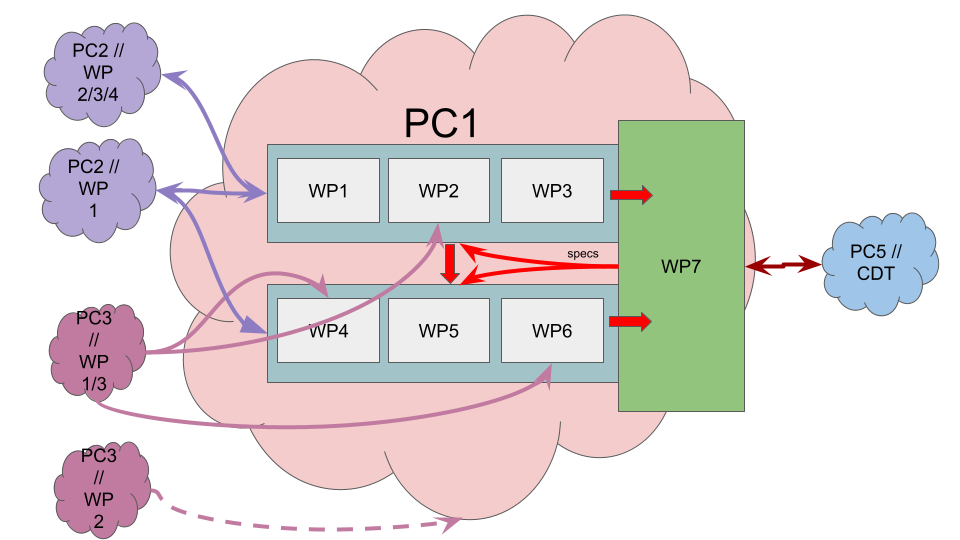
\includegraphics[width=.86\linewidth]{../../figures/exama-pc.png}

\end{frame}


\subsection{Governance}
\begin{frame}
  \frametitle{\insertsectionhead}
  \framesubtitle{\insertsubsectionhead}

Governance:
\begin{itemize}
  \item Steering committee: Pilots+WP leaders
  \item Scientific advisory board (European, American and possibly Asian)
\end{itemize}

\end{frame}

\section*{External Partners}

\begin{frame}[plain]
  \frametitle{}
  \framesubtitle{}
\begin{center}
  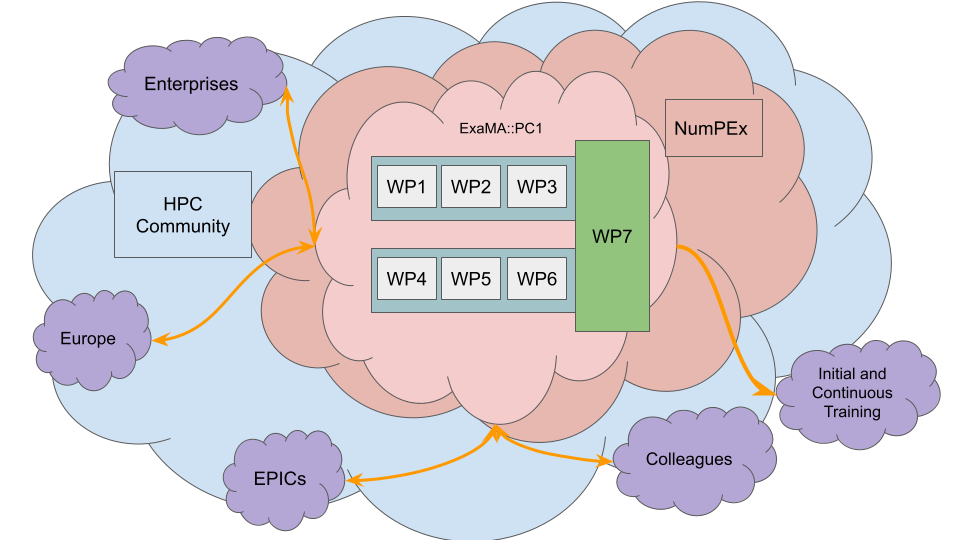
\includegraphics[width=.9\linewidth]{../../figures/exama-relations.png}
\end{center}
  
\end{frame}

\begin{frame}
  \frametitle{\insertsectionhead}
  \framesubtitle{\insertsubsectionhead}

  Setting up this network and creating a group of external partners, we will succeed in
  \begin{itemize}
    \item bringing together our community to solve scientific challenges to move to the Exascale
    \item jointly develop software bricks to scale up to Exascale
    \item creating/strengthening collaborations between external partners and Exa-MA partners 
    \item better structuring our community to respond effectively to European and international calls for projects.
  \end{itemize}

\end{frame}
\begin{frame}
  \frametitle{\insertsectionhead}
  \framesubtitle{\insertsubsectionhead}
  \begin{alertblock}{}
    \begin{itemize}
      \item Entreprises: TotalEnergies, Cerfacs, EdF
      \item EPIC: Onera, Ifpen
      \item Academia: UPPA, AMU, UL, TGIR-LNCMI
      \item European projects : CoE Hidalgo2
      \item International collaborations : U Luxembourg, CNR Italy
    \end{itemize}

    \href{https://docs.google.com/spreadsheets/d/1SpvhxFXcr8HfSSdlsU3lIMl73_KH7xFBa65yokAUHdk/edit?usp=sharing}{\beamerbutton{> External Partners}}
  \end{alertblock}


\end{frame}

\begin{frame}
  \frametitle{Tools}

  External partners will not receive direct funding, BUT the following tools are at our disposal

\begin{itemize}
  \item Co-funding activities (PhD, post-doc, engineers, etc.)
  \item Collaboration through co-supervision of PhD students and post-docs
  \item Collaboration through software developments
  \item Collaboration through Use Cases
  \item Co-organization of events
  \item Consortium creation for European and international projects
  \item Regular communication on the project and its advances
  \item Participation to ExaMA and NumPEx events
\end{itemize}

\begin{alertblock}{External Partners}
 We would like to propose a specific statute and representation of external partners.
\end{alertblock}
  
\end{frame}


\begin{frame}
  \frametitle{Statute}
  
  Gouvernance of ExaMA:
  \begin{itemize}
    \item Steering committee : PC1 pilots, PC1 WP leaders and representants of NumPEx 
    \item Scientific advisory committee (european and international)
    \item \alert{External partners board with both institutional and scientific representatives}
  \end{itemize}

\end{frame}
